\documentclass[a4paper]{article}
\usepackage[T1]{fontenc}			% \chapter package
\usepackage[english]{babel}
\usepackage[english]{isodate}  		% date format
\usepackage{graphicx}				% manage images
\usepackage{amsfonts}
\usepackage{booktabs}				% high quality tables
\usepackage{amsmath}				% math package
\usepackage{amssymb}				% another math package (e.g. \nexists)
\usepackage{bm}                     % bold math symbols
\usepackage{mathtools}				% emphasize equations
\usepackage{stmaryrd} 				% '\llbracket' and '\rrbracket'
\usepackage{amsthm}					% better theorems
\usepackage{enumitem}				% manage list
\usepackage{pifont}					% nice itemize
\usepackage{cancel}					% cancel math equations
\usepackage{caption}				% custom caption
\usepackage[]{mdframed}				% box text
\usepackage{multirow}				% more lines in a table
\usepackage{textcomp, gensymb}		% degree symbol
\usepackage[x11names]{xcolor}		% RGB color
\usepackage[many]{tcolorbox}		% colorful box
\usepackage{multicol}				% more rows in a table (used for the lists)
\usepackage{listings}
\usepackage{url}
\usepackage{qrcode}
\usepackage{fontawesome5}
\usepackage{ragged2e}
\usepackage{cite}                   % references
\usepackage{imakeidx}               % index
\makeindex[program=makeindex, columns=1,
           title=Index, 
           intoc,
           options={-s index-style.ist}]
\usepackage{fancyhdr}
\usepackage{eurosym}                % Euro symbol package
\usepackage{moreverb}               % verbatim to fix white lines in code snippets (mathescape problem with lstlisting)

%\pdfcompresslevel=0
%\pdfobjcompresslevel=0

\definecolor{codegreen}{rgb}{0,0.6,0}
\definecolor{codegray}{rgb}{0.5,0.5,0.5}
\definecolor{codepurple}{rgb}{0.58,0,0.82}
%\definecolor{backcolour}{rgb}{0.95,0.95,0.92}
\definecolor{backcolour}{rgb}{255,255,255}
\lstdefinestyle{mystyle}{
	backgroundcolor=\color{backcolour},   
	commentstyle=\color{codegreen},
	keywordstyle=\color{magenta},
	numberstyle=\tiny\color{codegray},
	stringstyle=\color{codepurple},
	basicstyle=\ttfamily\footnotesize,
	breakatwhitespace=false,         
	breaklines=true,                 
	captionpos=b,                    
	keepspaces=true,                 
	numbers=left,                    
	numbersep=5pt,                  
	showspaces=false,                
	showstringspaces=false,
	showtabs=false,                  
	tabsize=2,
    mathescape,
    frame=lines
}

\lstdefinelanguage{pseudo-code}{
	keywords={while, do, for, if, and, then},
	keywordstyle=\color{Red2}\bfseries,
	ndkeywords={},
	ndkeywordstyle=\color{darkgray}\bfseries,
	identifierstyle=\color{black},
	sensitive=false,
	comment=[l]{//},
	morecomment=[s]{/*}{*/},
	commentstyle=\color{codegreen}\ttfamily,
	stringstyle=\color{red}\ttfamily,
	morestring=[b]',
	morestring=[b]"
}

\lstset{
	language=pseudo-code,
	backgroundcolor=\color{lightgray},
	extendedchars=true,
	basicstyle=\footnotesize\ttfamily,
	showstringspaces=false,
	showspaces=false,
	numbers=left,
	numberstyle=\footnotesize,
	numbersep=9pt,
	tabsize=2,
	breaklines=true,
	showtabs=false,
	captionpos=b
}

\lstset{style=mystyle}


% thanks Mico: https://tex.stackexchange.com/a/60218/312896
\makeatletter
\renewcommand\paragraph{\@startsection{paragraph}{4}{\z@}%
            {-2.5ex\@plus -1ex \@minus -.25ex}%
            {1.25ex \@plus .25ex}%
            {\normalfont\normalsize\bfseries}}
\makeatother
\setcounter{secnumdepth}{4} % how many sectioning levels to assign numbers to
\setcounter{tocdepth}{4}    % how many sectioning levels to show in ToC


% draw a frame around given text
\newcommand{\framedtext}[1]{%
	\par%
	\noindent\fbox{%
		\parbox{\dimexpr\linewidth-2\fboxsep-2\fboxrule}{#1}%
	}%
}


% table of content links
\usepackage{xcolor}
\usepackage[linkcolor=black, citecolor=blue, urlcolor=cyan]{hyperref} % hypertexnames=false
\hypersetup{
	colorlinks=true
}


\newtheorem{theorem}{\textcolor{Red3}{\underline{Theorem}}}
\renewcommand{\qedsymbol}{QED}
\newcommand{\dquotes}[1]{``#1''}
\newcommand{\longline}{\noindent\rule{\textwidth}{0.4pt}}
\newcommand{\circledtext}[1]{\raisebox{.5pt}{\textcircled{\raisebox{-.9pt}{#1}}}}
\newcommand{\definition}[1]{\textcolor{Red3}{\textbf{#1}}\index{#1}}
\newcommand{\definitionWithSpecificIndex}[2]{\textcolor{Red3}{\textbf{#1}}\index{#2}}
\newcommand{\example}[1]{\textcolor{Green4}{\textbf{#1}}}
\newcommand{\highspace}{\vspace{1.2em}\noindent}
\newcommand{\opt}{\mathrm{opt} \:}
\renewcommand{\lstlistingname}{Algorithm}
\renewcommand{\lstlistlistingname}{Algorithms}
\newcommand{\version}{v0.4.1}


\begin{document}
    \newcounter{definition}[section]
    \newcounter{example}[section]
    \newcounter{exercise}[section]
    
    \newtcolorbox[use counter = definition]{definitionbox}[1][]{%
        breakable,
        enhanced,
        colback=red!5!white,
        colframe=red!75!black,
        fonttitle=\bfseries,
        title={Definition \thetcbcounter#1} %
    }

    \newtcolorbox[use counter = exercise]{exercisebox}[1][]{%
        breakable,
        enhanced,
        colback=Red3!5!white,
        colframe=Red3!75!black,
        fonttitle=\bfseries,
        title={Exercise \thetcbcounter#1} %
    }
    
    \newtcolorbox[use counter = example]{examplebox}[1][]{%
        breakable,
        enhanced,
        colback=Green4!5!white,
        colframe=Green4!75!black,
        fonttitle=\bfseries,
        title={Example \thetcbcounter#1} %
    }

    \newtcolorbox[]{deepeningbox}[1][]{%
        breakable,
        enhanced,
        colback=DarkOrange3!5!white,
        colframe=DarkOrange3!75!black,
        fonttitle=\bfseries,
        title={Deepening#1} %
    }

    %%%%%%%%%%%%%%%
    % Notes cover %
    %%%%%%%%%%%%%%%
    \author{260236}
\title{Parallel Computing - Notes - \version}
\date{\printdayoff\today}
\maketitle

    %%%%%%%%%%%
    % Preface %
    %%%%%%%%%%%
	\section*{Preface}

Every theory section in these notes has been taken from the sources:
\begin{itemize}
    \item Course slides.\cite{numerical-linear-algebra-polimi}
\end{itemize}
About:
\begin{itemize}
    \item[\faIcon{github}] \href{https://github.com/PoliMI-HPC-E-notes-projects-AndreVale69/HPC-E-PoliMI-university-notes}{GitHub repository}
    \begin{center}
        \qrcode{https://github.com/PoliMI-HPC-E-notes-projects-AndreVale69/HPC-E-PoliMI-university-notes}
    \end{center}
\end{itemize}
These notes are an unofficial resource and shouldn't replace the course material or any other book on numerical linear algebra. It is not made for commercial purposes. I've made the following notes to help me improve my knowledge and maybe it can be helpful for everyone.

As I have highlighted, a student should choose the teacher's material or a book on the topic. These notes can only be a helpful material.

\highspace

\subsection*{Correlated Projects}

During the Numerical Linear Algebra for HPC course, I was part of a team where we created a project that included two challenges related to the course. See more details in the corresponding repository:
\begin{itemize}
    \item[\faIcon{github}] \href{https://github.com/PoliMI-HPC-E-notes-projects-AndreVale69/NLA-challenges}{GitHub repository}
    \begin{center}
        \qrcode{https://github.com/PoliMI-HPC-E-notes-projects-AndreVale69/NLA-challenges}
    \end{center}
\end{itemize}

    %%%%%%%%%%%%%%%%%%%%%
    % Table of contents %
    %%%%%%%%%%%%%%%%%%%%%
    \tableofcontents
    \newpage

    %%%%%%%%%%%%
    % Listings %
    %%%%%%%%%%%%
    \lstlistoflistings

    %%%%%%%%%%%%%%%%
    % Introduction %
    %%%%%%%%%%%%%%%%
    \section{Introduction}

\begin{definitionbox}
    \definition{Operations Research (OR)}, often shortened to the initialism \texttt{OR}, is the branch of mathematics in which \textbf{mathematical models} and \textbf{quantitative methods} (e.g. optimization, game theory, simulation) are \textbf{used to analyze complex decision-making problems} and \textbf{find (near-)optimal solutions}.
\end{definitionbox}

\highspace
The overall and primary \emph{goal} is to \emph{help make better decisions}.

\highspace
OR can be seen as an interdisciplinary field at the intersection of applied mathematics, computer science, economics, and industrial engineering.

\highspace
Operations research is often concerned with \textbf{determining the extreme values of some real-world objective}: the \emph{maximum} (of profit, performance, or yield) or \emph{minimum} (of loss, risk, or cost). Originating in military efforts before World War II, its techniques have grown to concern problems in a variety of industries.\cite{wikipediaOperationsResearch}

\longline

\subsection{Decision-making problems}

Decision-making problems are analyzed using mathematical models and quantitative methods.

\begin{definitionbox}
    \definition{Decision-making problems} are problems in which we must \textbf{choose} a (feasible) \textbf{solution among a large number of alternatives based on one or several criteria}.
\end{definitionbox}

\highspace
Some practical \example{examples} include network design, shortest paths, staff scheduling, and service management.

\highspace
In other words, they are complex decision-making problems that are \textbf{addressed through a mathematical modeling approach} (mathematical models, algorithms, and computer implementations).
    \subsection{Scheme of an OR study}

The most important and common \textbf{steps} in operational research are:
\begin{enumerate}
    \item \textbf{Problem}. Define the problem;
    \item \textbf{Model}. Build the model;
    \item \textbf{Algorithm}. Select or develop an appropriate algorithm;
    \item \textbf{Implementation}. Implementing or using an efficient computer program;
    \item \textbf{Results}. Analyze the results.
\end{enumerate}

\begin{definitionbox}
    A mathematical \definition{model} is a \textbf{simplified representation of a real-world problem}.
\end{definitionbox}

\noindent
To define a mathematical model, it is necessary to identify the fundamental elements of the problem and the main relationships between them. But \textbf{how can we decide} the \emph{number of decision makers}, the \emph{number of objectives} and the \emph{level of uncertainty in the parameters}? It depends on the environment. If we have:
\begin{itemize}
    \item One decision maker, one object, then we will use \textbf{mathematical programming}.
    \item One decision maker, multiple objectives, then we will use \textbf{multi-objective programming}.
    \item Uncertainty greater than zero, then we will use \textbf{stochastic programming}.
    \item Multiple decision makers, then we will use \textbf{game theory}.
\end{itemize}

\highspace
\begin{examplebox}[: production planning]
    A company produces 3 types of electronic devices: $D_{1}$, $D_{2}$, $D_{3}$; going through 3 main phases of the production process: assembly, refinement and quality control.

    Time (in minutes) required for each phase and product:

    \begin{center}
        \begin{tabular}{@{} c | c c c @{}}
            & $D_{1}$ & $D_{2}$ & $D_{3}$ \\
            \midrule
            Assembly        & $80$ & $70$ & $120$ \\
            Refinement      & $70$ & $90$ & $20$ \\
            Quality control & $40$ & $30$ & $20$
        \end{tabular}
    \end{center}

    Available resources within the planning horizon (depend on the workforce) in minutes:
    \begin{center}
        \begin{tabular}{@{} c | c | c @{}}
            Assembly & Refinement & Quality control \\
            \midrule
            $30'000$ & $25'000$ & $18'000$
        \end{tabular}
    \end{center}

    Unitary profit (in KEuro):
    \begin{center}
        \begin{tabular}{@{} c | c | c @{}}
            $D_{1}$ & $D_{2}$ & $D_{3}$ \\
            \midrule
            $1.6$ & $1$ & $2$
        \end{tabular}
    \end{center}
    
    Assumption: the company can sell whatever it produces.

    \emph{Give a mathematical model for determining a production plan which maximizes the total profit.}

    \begin{itemize}
        \item \textbf{Decision variables}, $x_{j}$ is equal to the number of devices $D_{j}$ produced, for $j = 1, 2, 3$.
        
        \item \textbf{Objective function}: $\max \: z = 1.6x_{1} + 1x_{2} + 2x_{3}$.

        \item \textbf{Constraints}: the production capacity limit for each phase:
        \begin{equation*}
            \begin{array}{rcl}
                80x_{1} + 70x_{2} + 120x_{3} &\le& 30'000 \hspace{2em} \text{(assembly)} \\ [.5em]
                70x_{1} + 90x_{2} + 20x_{3} &\le& 25'000 \hspace{2em} \text{(refinement)} \\ [.5em]
                40x_{1} + 30x_{2} + 20x_{3} &\le& 18'000 \hspace{2em} \text{(quality control)}
            \end{array}
        \end{equation*}

        \item \textbf{Non-negative variables}: $x_{1}, x_{2}, x_{3} \ge 0$ may be fractional (real) values.
    \end{itemize}
\end{examplebox}

\begin{examplebox}[: portfolio selection problem]
    An insurance company must decide which investments to select out of a given set of possible assets (stocks, bonds, options, gold certificates, real estate, \dots).

    \begin{center}
        \begin{tabular}{@{} c | c c c @{}}
            Investments & area & capital $\left(c_{j} \: K€\right)$ & expected return $\left(r_{j}\right)$ \\
            \midrule
            A & Germany & $150$ & $11\%$ \\
            B & Italy & $150$ & $9\%$ \\
            C & U.S.A. & $60$ & $13\%$ \\
            D & Italy & $100$ & $10\%$ \\
            E & Italy & $125$ & $8\%$ \\
            F & France & $100$ & $7\%$ \\
            G & Italy & $50$ & $3\%$ \\
            H & UK & $80$ & $5\%$
        \end{tabular}
    \end{center}
    Legend:
    \begin{itemize}
        \item A and B: automotive
        \item C and D: ICT
        \item E and F: real estate
        \item G: short term treasury bounds
        \item H: long term treasury bounds
    \end{itemize}
    The available capital is: $600$ KEuro.

    At most 5 investments to avoid excessive fragmentation.

    Geographic diversification to limit risk: $\le 3$ investments in Italy and $\le 3$ abroad.

    \emph{Give a mathematical model for deciding which investments to select so as to maximize the expected return while satisfying the constraints.}

    \begin{itemize}
        \item \textbf{Decision variables}, $x_{j}$ is equal to $1$ if $j$-th investment is selected and $x_{j}=0$ otherwise, for $j = 1, \dots, 8$.
        
        \item \textbf{Objective function}: $\max \: z = \displaystyle\sum_{j=1}^{8} c_{j} \: r_{j} \: x_{j}$.

        \item \textbf{Constraints}:
        \begin{equation*}
            \begin{array}{rclcl}
                \displaystyle\sum_{j=1}^{8}c_{j} \: x_{j} &\le& 600 &\hspace{1em}& \text{(capital)} \\ [2em]
                \displaystyle\sum_{j=1}^{8}x_{j} &\le& 5 &\hspace{1em}& \text{(max 5 investments)} \\ [2em]
                x_{2}+x_{4}+x_{5}+x_{7} &\le& 3 &\hspace{1em}& \text{(max 3 in Italy)} \\ [.5em]
                x_{1}+x_{3}+x_{6}+x_{8} &\le& 3 &\hspace{1em}& \text{(max 3 abroad)}
            \end{array}
        \end{equation*}

        \item \textbf{Binary (integer) variables}: $x_{j} \in \left\{0,1\right\}$ and $1 \le j \le 8$.
    \end{itemize}

    \underline{\textbf{Possible variant}}. In order to limit the risk, if any of the ICT investment is selected then at least one of the treasury bond must be selected.
    \begin{itemize}
        \item \textbf{Objective function}: $\max z = \displaystyle\sum_{j=1}^{8} c_{j} \: r_{j} \: x_{j}$.

        \item \textbf{Constraints}:
        \begin{equation*}
            \begin{array}{rcll}
                \displaystyle\sum_{j=1}^{8}c_{j} \: x_{j} &\le& 600 & \text{(capital)} \\ [2em]
                \displaystyle\sum_{j=1}^{8}x_{j} &\le& 5 & \text{(max 5 investments)} \\ [2em]
                x_{2}+x_{4}+x_{5}+x_{7} &\le& 3 & \text{(max 3 in Italy)} \\ [.5em]
                x_{1}+x_{3}+x_{6}+x_{8} &\le& 3 & \text{(max 3 abroad)} \\ [1em]
                \dfrac{x_{3} + x_{4}}{2} &\le& x_{7} + x_{8} & \text{(investment in treasury bonds)}
            \end{array}
        \end{equation*}

        \item \textbf{Binary (integer) variables}: $x_{j} \in \left\{0,1\right\}$ and $1 \le j \le 8$.
    \end{itemize}
\end{examplebox}

\newpage

\begin{examplebox}[: facility location]
    Consider 3 oil pits, located in positions $A$, $B$ and $C$, from which oil is extracted.

    \begin{center}
        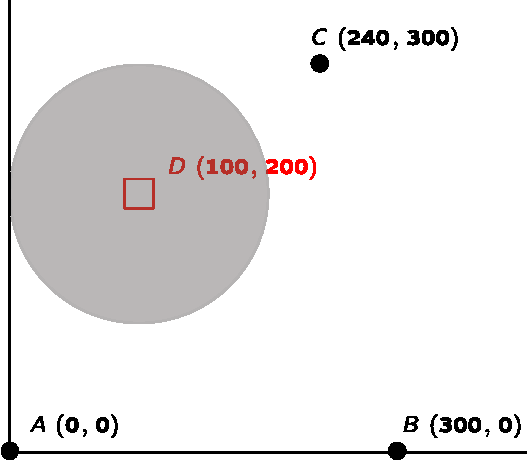
\includegraphics[width=.6\textwidth]{img/facility-location-1.pdf}
    \end{center}

    Connect them to a refinery with pipelines whose cost is proportional to the square of their length.

    The refinery must be at least 100 km away from point $D = \left(100, 200\right)$, but the oil pipelines can cross the corresponding forbidden zone.

    \emph{Give a mathematical model to decide where to locate the refinery so as to minimize the total pipeline cost.}

    \begin{itemize}
        \item \textbf{Decision variables}, $x_{1}, x_{2}$ cartesian coordinates of the refinery.
        
        \item \textbf{Objective function}:
        \begin{equation*}
            \begin{array}{rl}
                \min z = & \left[\left(x_{1} - 0\right)^{2} + \left(x_{2} - 0\right)^{2}\right] + \\ [.5em]
                         & \left[\left(x_{1} - 300\right)^{2} + \left(x_{2} - 0\right)^{2}\right] + \\ [.5em]
                         & \left[\left(x_{1} - 240\right)^{2} + \left(x_{2} - 300\right)^{2}\right]
            \end{array}
        \end{equation*}

        \item \textbf{Constraints}:
        \begin{equation*}
            \sqrt{
                \left(x_{1}-100\right)^{2} + \left(x_{2} - 200\right)^{2}
            } \ge 100
        \end{equation*}

        \item \textbf{Variables}: $x_{1}, x_{2} \in \mathbb{R}$.
    \end{itemize}
\end{examplebox}
    \subsection{Mathematical programming/optimization}

\definition{Mathematical Optimization} or \definition{Mathematical Programming} is the \textbf{selection of a best element}, with regard to some criteria, \textbf{from some set of available alternatives}.

In the more general approach, an optimization problem consists of \textbf{maximizing} or \textbf{minimizing a real function} by systematically choosing input values from within an allowed set and computing the value of the function. The generalization of optimization theory and techniques to other formulations constitutes a large area of applied mathematics.

\highspace
\begin{flushleft}
    \textcolor{Green3}{\faIcon{question-circle} \textbf{And where should we start?}}
\end{flushleft}
Decision-making problems are characterized by a \textbf{single decision maker}, a \textbf{single objective}, and \textbf{reliable parameter estimates}. Using mathematical language, we can say:
\begin{equation*}
    \opt f\left(\mathbf{x}\right) \hspace{1em} \text{with} \hspace{1em} \mathbf{x} \in X \hspace{1em} \text{and} \hspace{1em} \opt = \begin{Bmatrix}
        \min \\ \max
    \end{Bmatrix}
\end{equation*}
Where:
\begin{itemize}
    \item $\mathbf{x} \in \mathbb{R}^{n}$ \textbf{decision variables}. They are numerical variables whose values identify a solution of the problem.

    \item $X \subseteq \mathbb{R}^{n}$ \textbf{feasible region}. Distinguishes between feasible and infeasible solutions (via constraints):
    \begin{equation*}
        X = \left\{\mathbf{x} \in \mathbb{R}^{n} \: : \: g_{i}\left(\mathbf{x}\right) \begin{Bmatrix}
        = \\ \le \\ \ge
        \end{Bmatrix} 0, i = 1, \dots, m\right\}
    \end{equation*}

    \item $f: X \rightarrow \mathbb{R}$ \textbf{objective function}.Expresses in quantitative terms the value or cost of each feasible solution.
\end{itemize}
Note an interesting observation:
\begin{equation*}
    \max\left\{f\left(\mathbf{x}\right): \: \mathbf{x} \in X\right\} = -\min\left\{-f\left(\mathbf{x}\right): \: \mathbf{x} \in X\right\}
\end{equation*} 
    \subsection{Multi-objective programming}\label{subsection: Multi-objective programming}

\begin{flushleft}
    \textcolor{Green3}{\faIcon{question-circle} \textbf{How is it born?}}
\end{flushleft}
Even though some real-word problems can be reduced to a matter of a single objective very often it is hard to define all the aspects in terms of a single objective. Defining multiple objectives often gives a better idea of the task.

\highspace
\definition{Multi-objective programming} (also known as \definition{Multi-objective optimization} or \definition{Pareto optimization}) is an \textbf{area of multiple-criteria decision making} that is concerned with mathematical optimization problems involving \textbf{more than one objective function to be optimized simultaneously}. Multi-objective is a type of vector optimization that has been applied in many fields of science, including engineering, economics and logistics where optimal decisions need to be taken in the presence of trade-offs between two or more conflicting objectives. 

Minimizing cost while maximizing comfort while buying a car, and maximizing performance whilst minimizing fuel consumption and emission of pollutants of a vehicle are \example{examples} of multi-objective optimization problems involving two and three objectives, respectively.\cite{abraham2005evolutionary}

\highspace
Suppose to minimize $f_{1}\left(\mathbf{x}\right)$ and maximize $f_{2}\left(\mathbf{x}\right)$ (e.g. laptop: $f_{1}$ is cost and $f_{2}\left(\mathbf{x}\right)$ is performance):
\begin{enumerate}
    \item Turn it into a \definition{single objective problem} by expressing the two objectives in terms of the same unit (e.g. monetary unit):
    \begin{equation*}
        \min \lambda_{1}f_{1}\left(\mathbf{x}\right) - \lambda_{2}f_{2}\left(\mathbf{x}\right)
    \end{equation*}
    for appropriate scalars $\lambda_{1}$ and $\lambda_{2}$.

    \item Optimize the \definition{primary objective} function and turn the other objective into a constraint:
    \begin{equation*}
        \underset{x \in \tilde{X}}{\max} f_{2}\left(\mathbf{x}\right) \hspace{1em} \text{where} \hspace{1em} \tilde{X} = \left\{\mathbf{x} \in X \: : \: f_{1}\left(\mathbf{x}\right) \le \varepsilon \right\}
    \end{equation*}
    for appropriate constant $\varepsilon$.
\end{enumerate}
This is a simple introduction, the more detailed explanation will be explained in the following pages.
    \subsection{Mathematical Programming or Simulation?}

Mathematical Programming and Simulation involves \textbf{building a model} and \textbf{designing an algorithm}. And the main differences are:
\begin{table}[!htp]
    \centering
    \begin{tabular}{@{} p{15em} | p{15em} @{}}
        \toprule
        \textbf{Mathematical Programming} & \textbf{Simulation} \\
        \midrule
        Problem can be \dquotes{well} formalized. & Problem is difficult to formalize. \\
        \cmidrule{1-2}
        Algorithm yields a(n optimal) solution. & Algorithm simulates the evolution of the real system and allows to evaluate the performance of alternative solutions. \\
        \cmidrule{1-2}
        The results are \dquotes{certain} & The results need to be interpreted. \\
        \cmidrule{1-2}
        Example: assignment. & Example: service counters. \\
        \bottomrule
    \end{tabular}
    \caption{Major differences between Mathematical Programming and Simulation.}
\end{table}

    %%%%%%%%%%%%%%%%%%%%%%%%%%%%%%%%%%
    % Graph and network optimization %
    %%%%%%%%%%%%%%%%%%%%%%%%%%%%%%%%%%
    \section{Graph and network optimization}

\subsection{Graphs}

\subsubsection{Definitions and characteristics}

In the following section we will explain some basic concepts about the graphs. The terms used are important, and we will use the definition box to highlight these words.

\highspace
\begin{definitionbox}[: graph]
    A \definitionWithSpecificIndex{graph}{Graph} is a pair $G = \left(N,E\right)$, with $N$ a set of \textbf{nodes} or \textbf{vertices} and $E \subseteq N \times N$ a set of \textbf{edges} or \textbf{arcs} connecting them pairwise.
\end{definitionbox}

\highspace
\begin{definitionbox}[: edge]
    An \definitionWithSpecificIndex{edge}{Edge} connecting the nodes $i$ and $j$ is represented by
    \begin{itemize}
        \item Graph undirected: $\left\{i,j\right\}$
        \item Graph directed: $\left(i,j\right)$
    \end{itemize}
\end{definitionbox}

\highspace
\begin{examplebox}
    For \example{example}, a road network which connects $n$ cities can be modelled, by a graph where a city corresponds to a node, and a connection corresponds to an edge.

    \begin{center}
        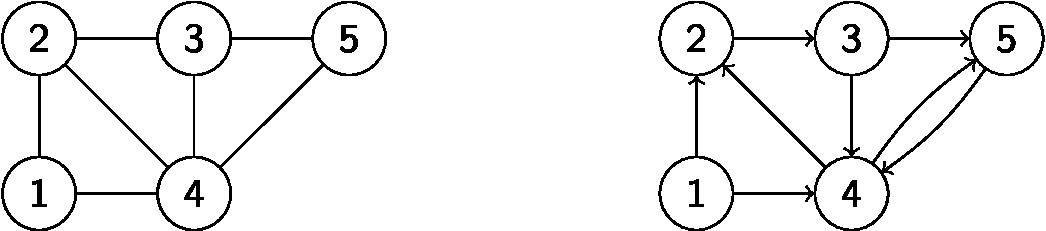
\includegraphics[width=.8\textwidth]{img/graphs-1.pdf}
    \end{center}

    \noindent
    \begin{itemize}
        \item Undirected graph:
        \begin{itemize}
            \item $N = \left\{1,2,3,4,5\right\}$
            \item $E = \left\{
                \left\{1,2\right\},
                \left\{1,4\right\},
                \left\{2,3\right\},
                \left\{2,4\right\},
                \left\{3,4\right\},
                \left\{3,5\right\},
                \left\{4,5\right\}
            \right\}$
        \end{itemize}
        
        \item Directed graph:
        \begin{itemize}
            \item $N = \left\{1,2,3,4,5\right\}$
            \item $E' = \left\{
                \left(1,2\right),
                \left(1,4\right),
                \left(2,3\right),
                \left(2,4\right),
                \left(3,4\right),
                \left(3,5\right),
                \left(4,5\right)
            \right\}$
        \end{itemize}
    \end{itemize}
\end{examplebox}

\newpage

\noindent
Some graph properties are:
\begin{itemize}
    \item Two \textbf{nodes} are \definitionWithSpecificIndex{adjacent}{Adjacent nodes} if they are \textbf{connected by an edge}.

    \item An \textbf{edge} $e$ is \definitionWithSpecificIndex{incident}{Incident edge} in a node $v$ if $v$ is an endpoint of $e$.
    
    In other words, in a graph $G$, two edges are incident \textbf{if they share a common vertex}. For example, edge $E_{1}=\left(v_{1}, v_{2}\right)$ and edge $\left(v_{1}, v_{3}\right)$ are incident as they share the same vertex $v_{1}$.

    \item The degree concept depends on the type of graph:
    \begin{itemize}
        \item Undirected graph: the \definitionWithSpecificIndex{degree}{Node degree} of a node is the \textbf{number of incident edges}.

        \item Directed graph: the \definitionWithSpecificIndex{in-degree}{Node in-degree} and \definitionWithSpecificIndex{out-degree}{Node out-degree} of a node is the \textbf{number of arcs that have it as succesor} and \textbf{predecessor}.
    \end{itemize}
\end{itemize}

\highspace
\begin{examplebox}[: adjacent, incident, degree, in-degree and out-degree]
    Given the graphs:
    
    \begin{center}
        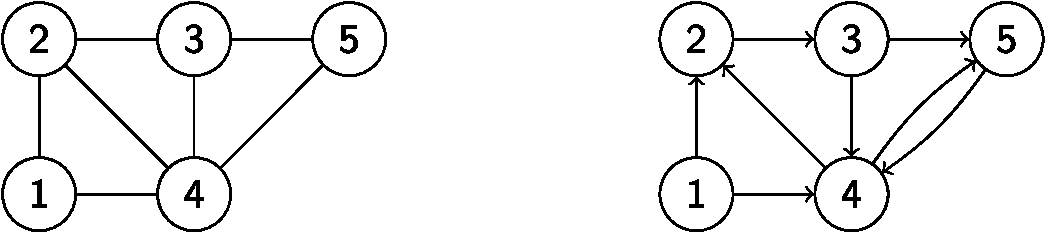
\includegraphics[width=.8\textwidth]{img/graphs-2.pdf}
    \end{center}

    \begin{itemize}
        \item Undirected graph:
        \begin{itemize}
            \item Nodes 1 and 2 are \textbf{adjacent} (unlike nodes 1 and 3).
            \item Edge $\left\{1,2\right\}$ is \textbf{incident} in nodes 1 and 2.
            \item Node 1 has \textbf{degree} 2, node 4 has \textbf{degree} 4.
        \end{itemize}

        \item Directed graph: node 1 has \textbf{in-degree} 0, and \textbf{out-degree} 2.
    \end{itemize}
\end{examplebox}

\highspace
Other useful features include:
\begin{itemize}
    \item A \definitionWithSpecificIndex{(directed) path from $i \in N$ to $j \in N$}{Directed path from $i \in N$ to $j \in N$} is a sequence of (arcs) edges:
    \begin{equation*}
        p = \left\langle \left\{v_{1}, v_{2}\right\}, \left\{v_{2}, v_{3}\right\}, \dots, \left\{v_{k-1}, v_{k}\right\} \right\rangle
    \end{equation*}
    Connecting nodes $v_{1}$ and $v_{k}$, with $\left\{v_{i}, v_{i+1}\right\} \in E$, for $i = 0, \dots, k-1$.

    \item A generic \textbf{node} $u$ and $v$ are \definitionWithSpecificIndex{connected}{Connected nodes} if there is a path connecting them.
    
    \item A \textbf{graph} $\left(N,E\right)$ is \definitionWithSpecificIndex{connected}{Connected graph} if two generic nodes $u,v$ are connected, $\forall u,v \in N$. Recall that in generic graph notation, the variable $N$ represents a set of nodes or vertices and $E$ represents a set of edges or arcs connecting them in pairs.
    
    \item A \textbf{graph} $\left(N,E\right)$ is \definitionWithSpecificIndex{strongly connected}{Strongly connected graph} if two generic nodes $u,v$ are connected by a directed path, $\forall u,v \in N$ (for any node in the set of nodes or vertices of the graph).
\end{itemize}

\highspace
\begin{examplebox}[: directed path, connected nodes, connected graph, strongly connected]
    Given the graphs:
    
    \begin{center}
        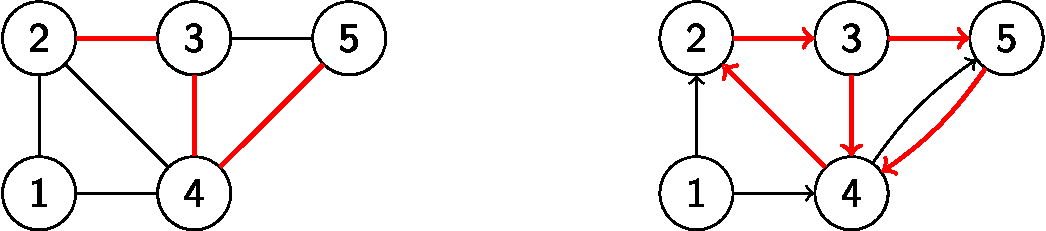
\includegraphics[width=.8\textwidth]{img/graphs-3.pdf}
    \end{center}

    \begin{itemize}
        \item Undirected graph:
        \begin{itemize}
            \item $\left\langle \left\{2,3\right\}, \left\{3,4\right\}, \left\{4,5\right\} \right\rangle$ is a \textbf{path} from node 2 to node 5.
            \item \textbf{Nodes} 2 and 5 are \textbf{connected}.
            \item It is a \textbf{connected graph}.
        \end{itemize}

        \item Directed graph:
        \begin{itemize}
            \item $\left\langle \left\{3,5\right\}, \left\{5,4\right\}, \left\{4,2\right\}, \left\{2,3\right\}, \left\{3,4\right\} \right\rangle$ is a \textbf{directed path} from node 3 to node 4.
            
            \item It is not a \textbf{strongly connected graph} because the node 1 cannot be the destination of none path. In other words, doesn't exist a directed path from node $u$ to node $1$ (where $u$ is a generic node, $\forall u \in N \setminus \left\{1\right\}$).
        \end{itemize}
    \end{itemize}
\end{examplebox}

\highspace
Finally, there are other interesting properties and notations about graphs and edges:
\begin{itemize}
    \item A \definitionWithSpecificIndex{cycle (circuit)}{Cycle in graph}\index{Circuit in graph} is a directed path with $v_{1} = v_{k}$ (source and destination are the same).

    \item A \textbf{graph} is \definitionWithSpecificIndex{bipartite}{Bipartite graph} if there is a partition $N = N_{1} \cup N_{2}$ $\left(N_{1} \cap N_{2} = \emptyset\right)$ such that no edge connects nodes in the same subset.

    \item A \textbf{graph} is \definitionWithSpecificIndex{complete}{Complete graph} if $E = \left\{\left\{v_{j}, v_{j}\right\} \: : \: v_{i}, v_{j} \in N \: \land \: i \le j\right\}$.

    \item Given a directed graph $G = \left(N,A\right)$ and $S \subset N$, the \definitionWithSpecificIndex{outgoing cut}{Outgoing cut} induced by $S$ is:
    \begin{equation*}
        \delta^{+}\left(S\right) = \left\{\left(u,v\right) \in A \: : \: u \in S \: \land : v \in N \subseteq S\right\}
    \end{equation*}
    The \definitionWithSpecificIndex{incoming cut}{Incoming cut} induced by $S$ is:
    \begin{equation*}
        \delta^{-}\left(S\right) = \left\{\left(u,v\right) \in A \: : \: v \in S \: \land : u \in N \subseteq S\right\}
    \end{equation*}
\end{itemize}

\newpage

\begin{examplebox}[: cycle/circuit in graph, bipartite graph, complete graph, out/incoming cut]
    An example of cycle in graph:
    
    \begin{center}
        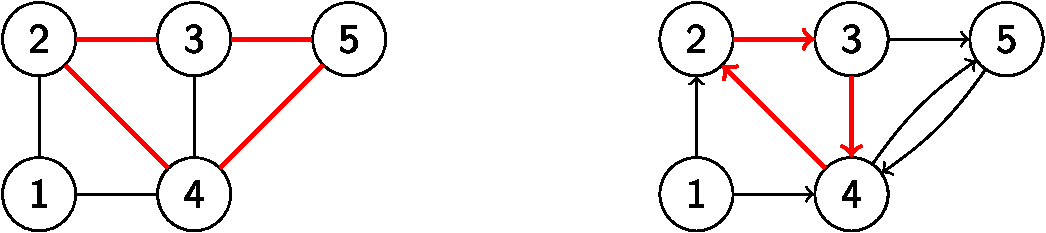
\includegraphics[width=.8\textwidth]{img/graphs-4.pdf}
    \end{center}

    \begin{itemize}
        \item Undirected graph: $\left\langle \left\{2,3\right\}, \left\{3,5\right\}, \left\{5,4\right\}, \left\{4,2\right\} \right\rangle$ is a cycle.
        \item Directed graph: $\left\langle \left(2,3\right), \left(3,4\right), \left(4,2\right) \right\rangle$ is a circuit.
    \end{itemize}
    %
    %

    An example of bipartite/complete graph:

    \begin{center}
        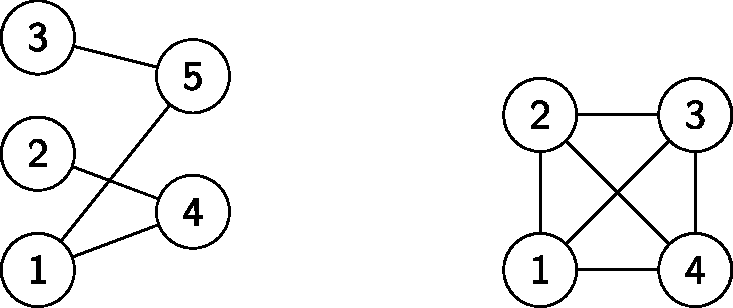
\includegraphics[width=.6\textwidth]{img/graphs-5.pdf}
    \end{center}

    \begin{itemize}
        \item To the left a \textbf{bipartite graph}, because:
        \begin{equation*}
            N_{1} = \left\{1,2,3\right\} \hspace{2em} N_{2} = \left\{4,5\right\}
        \end{equation*}
        \item And to the right a \textbf{complete graph}.
    \end{itemize}
    %
    %

    Finally, an example of out/incoming cut:
    
    \begin{center}
        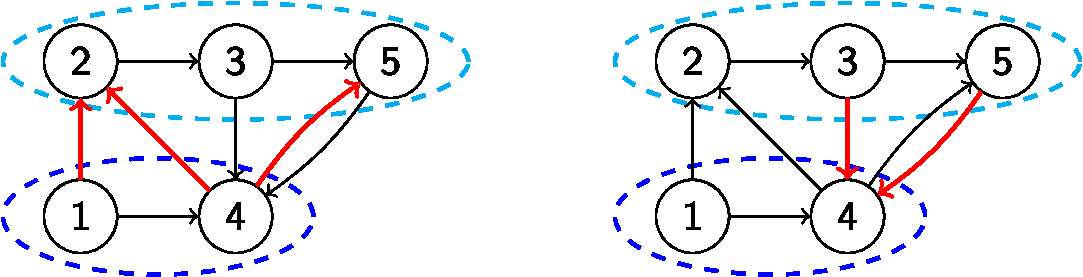
\includegraphics[width=.8\textwidth]{img/graphs-6.pdf}
    \end{center}

    \begin{itemize}
        \item Left graph: 
        \begin{equation*}
            \begin{array}{rcl}
                \delta^{+}\left(\left\{1,4\right\}\right) &=& \left(\left\{1,2\right\}, \left\{4,2\right\}, \left\{4,5\right\}\right) \\ [.5em]
                S &=& \left\{1,4\right\} \\ [.5em]
                N \setminus S &=& \left\{2,3,5\right\}
            \end{array}
        \end{equation*}

        \item Right graph: 
        \begin{equation*}
            \begin{array}{rcl}
                \delta^{-}\left(\left\{1,4\right\}\right) &=& \left(\left\{3,4\right\}, \left\{5,4\right\}\right) \\ [.5em]
                S &=& \left\{1,4\right\} \\ [.5em]
                N \setminus S &=& \left\{2,3,5\right\}
            \end{array}
        \end{equation*}
    \end{itemize}
\end{examplebox}

\subsubsection{Graphical representation}

Such a matrix can easily be represented as a graph. This guarantees that it can be stored efficiently in a computer. But to understand how to do this in general, it's important to understand some other important properties:
\begin{itemize}
    \item For any graph $G$ with $n$ nodes, the \textbf{number of edges} satisfies:
    \begin{itemize}
        \item $m \le \dfrac{n\left(n-1\right)}{2}$ if $G$ is undirected.
        \item $m \le n\left(n-1\right)$ if $G$ is directed.
    \end{itemize}

    \item A graph is \definitionWithSpecificIndex{dense}{Dense graph} if $m \approx n^{2}$ and \definitionWithSpecificIndex{sparse}{Sparse graph} if $m \ll n^{2}$. Where $m$ is the number of arcs and $n$ the number of nodes.

    \item For dense directed graphs, exist an \textbf{adjacency matrix} $A_{n \times n}$:
    \begin{equation*}
        \begin{cases}
            a_{ij} = 1 & \text{if } \left(i,j\right) \in A \\
            a_{ij} = 0 & \text{otherwise}
        \end{cases}
    \end{equation*}
\end{itemize}
To build the adjacency matrix it is necessary to create a \textbf{list of successors} for each node. In other words, for \textbf{each node} we need to write the \textbf{outgoing edges} and write the matrix.
\begin{equation*}
    A = \begin{bmatrix}
        0 & 1 & 0 & 1 & 0 \\
        0 & 0 & 1 & 0 & 0 \\
        0 & 0 & 0 & 1 & 1 \\
        0 & 1 & 0 & 0 & 1 \\
        0 & 0 & 0 & 1 & 0
    \end{bmatrix}
    \hspace{2em}
    \begin{array}{rcl}
        S\left(1\right) &=& \left\{2,4\right\} \\
        S\left(2\right) &=& \left\{3\right\} \\
        S\left(3\right) &=& \left\{4,5\right\} \\
        S\left(4\right) &=& \left\{2,5\right\} \\
        S\left(5\right) &=& \left\{4\right\}
    \end{array}
\end{equation*}
Each row represents a node, and we set the value 1 if the column index is a node that has the arc of the row node as its incoming edge. So row one (node one) has the value one in column two (node two) and column four (node four).

\longline

\subsubsection{Graph reachability problem}

In general the \definitionWithSpecificIndex{graph reachability problem}{Graph reachability problem} can be formulated as follows.

\begin{definitionbox}[: graph reachability problem]
    Given a directed graph $G = \left(N,A\right)$ and a node $s$, determine all the node that are reachable from $s$.
\end{definitionbox}

\noindent
Where $N$ is the set of nodes and $A$ is the set of edges.

\highspace
The problem takes:
\begin{itemize}
    \item As \textbf{input} a \emph{\textbf{graph}} $G = \left(N,A\right)$ described by the successor lists and node $s \in N$.
    
    \item As \textbf{output} produces a \emph{\textbf{subset}} $M \subseteq N$ \emph{\textbf{of nodes}} of the graph $G$ reachable from $s$.
\end{itemize}
Our goal is to devise an efficient algorithm that allows us to find all nodes reachable from $s$.

\newpage

\paragraph{Description and algorithm}

\begin{definitionbox}[: Breadth-First Search]
    \definition{Breadth-First Search (BFS)} is an \textbf{algorithm for searching a tree data structure for a node that satisfies a given property}. It starts at the tree root and explores all nodes at the present depth prior to moving on to the nodes at the next depth level. Extra memory, usually a queue, is needed to keep track of the child nodes that were encountered but not yet explored.
\end{definitionbox}

\begin{lstlisting}[language=pseudo-code, caption={Graph reachability problem: Breadth-First Search}]
Q $\leftarrow$ $\{$s$\}$; $\label{bfs: q-definition}$
M $\leftarrow$ $\emptyset$; $\label{bfs: m-definition}$
while Q $\ne$ $\emptyset$ do: $\label{bfs: while cycle}$
    u $\leftarrow$ node in Q; $\label{bfs: take an element from the queue}$
    Q $\leftarrow$ Q $\setminus$ $\{$u$\}$; $\label{bfs: remove the popped item from the queue}$
    // label u
    M $\leftarrow$ M $\cup$ $\{$u$\}$ $\label{bfs: labeled as explored}$
    for (u, v) $\in$ $\delta^{+}$ (u) do: $\label{bfs: for each tuple in outgoing cut}$
        if v $\notin$ M and v $\notin$ Q: $\label{bfs: if adjacent node is not in reachable set and not in the queue}$
            Q $\leftarrow$ Q $\cup$ $\{$v$\}$ $\label{bfs: add the node v to the queue}$
\end{lstlisting}

\begin{itemize}
    \item[Rows \ref{bfs: q-definition}-\ref{bfs: m-definition}.] Declare a queue \texttt{Q} containing the nodes reachable from the source \texttt{s} and \textbf{not yet processed}. It is managed as a FIFO (First-In First-Out) queue. By definition, we add the \texttt{s} node at the beginning because it is our entry point.
    
    Then we declare the set \texttt{M}. It represents the subset of nodes of the graph that are reachable from the source \texttt{s}. Obviously, it is empty at the beginning of the algorithm.

    \item[Row \ref{bfs: while cycle}.] The BFS algorithm continues to process the nodes until the queue is empty. As long as there is an element, it continues.
    
    \item[Rows \ref{bfs: take an element from the queue}-\ref{bfs: remove the popped item from the queue}.] Take a node from the queue \texttt{Q} and assign it to the variable \texttt{u}. Also remove the element \texttt{u} from the set \texttt{Q}. In other words, perform a difference operation between the sets \texttt{Q} and the set composed only of the element \texttt{u} ($\texttt{Q} \setminus \left\{\texttt{u}\right\}$).
    
    For example, in Python we can get the same result using the \href{https://docs.python.org/3/library/collections.html#collections.deque.popleft}{\texttt{popleft}} method of the \href{https://docs.python.org/3/tutorial/datastructures.html#using-lists-as-queues}{\texttt{deque} data structure}.

    \item[Row \ref{bfs: labeled as explored}.] Using the union between sets, add the visited node \texttt{u} to the subset \texttt{M} of reachable nodes. This operation is also called \dquotes{labeling} because you are \emph{labeling} a node as \emph{visited}.
    
    \item[Row \ref{bfs: for each tuple in outgoing cut}.] Iterate each tuple (node \texttt{u} just popped from the queue, node \texttt{v} adjacent to node \texttt{u}) in the outgoing cut set of node \texttt{u}.
    
    \item[Rows \ref{bfs: if adjacent node is not in reachable set and not in the queue}-\ref{bfs: add the node v to the queue}.] If the adjacent node \texttt{v} is not in the reachable set \texttt{M} and it is not in the queue (so it is not waiting to be evaluated), add the adjacent node \texttt{v} to \texttt{Q} using the union set operation.
\end{itemize}
As we said, the algorithm continues until the queue is not empty. Note that the queue is updated each time a neighboring node is found that is not already in the solution set (\texttt{M}).

\newpage

\paragraph{Complexity of algorithm}

\begin{flushleft}
    \textcolor{Green3}{\faIcon{clock} \textbf{BFS Algorithm - Time Complexity}}
\end{flushleft}
The BFS time complexity%
\footnote{In theoretical computer science, the time complexity is the computational complexity that describes the amount of computer time it takes to run an algorithm. Time complexity is commonly estimated by counting the number of elementary operations performed by the algorithm, supposing that each elementary operation takes a fixed amount of time to perform. Thus, the amount of time taken and the number of elementary operations performed by the algorithm are taken to be related by a constant factor. (\href{https://en.wikipedia.org/wiki/Time_complexity}{source})}
can be expressed as $O\left(\left|N\right|+\left|A\right|\right)$, since \textbf{every node and every edge will be explored in the \underline{worst case}}.
\begin{itemize}
    \item $\left|N\right|$ is the number of \textbf{nodes};
    \item $\left|A\right|$ is the number of \textbf{edges} in the graph.
\end{itemize}
Note that $O\left(\left|A\right|\right)$ may vary between $O\left(1\right)$ and $O\left(N^{2}\right)$, depending on how sparse the input graph is. For example, for \textbf{dense graphs}, exactly $O\left(N^{2}\right)$.

\highspace
\begin{flushleft}
    \textcolor{Green3}{\faIcon{memory} \textbf{BFS Algorithm - Space Complexity}}
\end{flushleft}
When the number of nodes (or vertices) in the graph is known ahead of time, and additional data structures are used to determine which vertices have already been added to the queue, the space complexity%
\footnote{The space complexity of an algorithm or a data structure is the amount of memory space required to solve an instance of the computational problem as a function of characteristics of the input. It is the memory required by an algorithm until it executes completely. This includes the memory space used by its inputs, called input space, and any other (auxiliary) memory it uses during execution, which is called auxiliary space. (\href{https://en.wikipedia.org/wiki/Space_complexity}{source})}
can be expressed as $O\left(\left|N\right|\right)$, where $\left|N\right|$ is the number of vertices. This is in addition to the space required for the graph itself, which may vary depending on the graph representation used by an implementation of the algorithm.

\highspace
In other words, the algorithm needs:
\begin{itemize}
    \item The \textbf{space to store} the set $N$, i.e. the \textbf{set of all nodes} in the graph.
    \item The \textbf{space to store the graph itself} depends on the implementation used.
\end{itemize}
    \subsection{Trees}

\subsubsection{Definitions and characteristics}

Before introducing what a tree is, it is necessary to understand what a subgraph is. Mathematically speaking, $G'= \left(N', E'\right)$ is a \definitionWithSpecificIndex{subgraph}{Subgraph} of $G = \left(N,E\right)$ if $N' \subseteq N$ and $E' \subseteq E$.

\highspace
A \definitionWithSpecificIndex{tree of the graph $G$}{Tree of a graph} is a connected and acyclic subgraph of $G$ and it is represented as $G_{T} = \left(N', T\right)$. If the tree contains exactly every node in the graph $G$, it is called the \definitionWithSpecificIndex{spanning tree}{Spanning tree} of $G$ and is represented as $G_{T} = \left(N', T\right)$. Finally, we call the \textbf{nodes of degree 1} in a tree as \definitionWithSpecificIndex{leaves}{Leaves of a tree}.

\begin{examplebox}[: subgraph, tree and spanning tree]
    Given a graph $G$:
    \begin{center}
        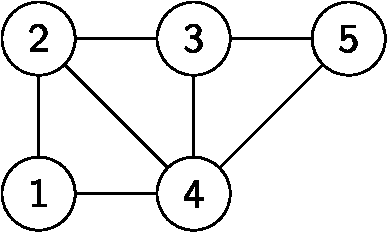
\includegraphics[width=.3\textwidth]{img/trees-1.pdf}
    \end{center}

    \begin{itemize}
        \item The following figure is a \textbf{subgraph} of $G$, but \underline{not} a tree, because there is a cycle $\left(1,2,4\right)$.
        \begin{center}
            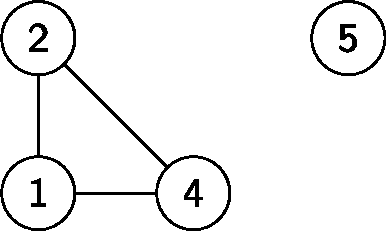
\includegraphics[width=.3\textwidth]{img/trees-2.pdf}
        \end{center}

        \item The following figure is a \textbf{subgraph} of $G$, and it is a \textbf{tree} because there are no cycles and the graph is connected.
        \begin{center}
            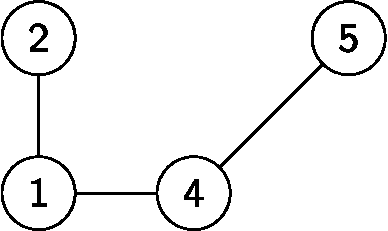
\includegraphics[width=.3\textwidth]{img/trees-3.pdf}
        \end{center}
        
        \item The following figure is a \textbf{spanning tree} of $G$ because it contains all the nodes in $G$, and it is a tree because it is connected and acyclic.
        \begin{center}
            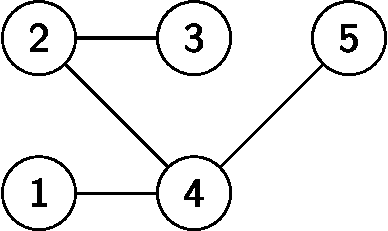
\includegraphics[width=.3\textwidth]{img/trees-4.pdf}
        \end{center}
    \end{itemize}
\end{examplebox}

\newpage

\subsubsection{Properties}

\begin{enumerate}
    \item \textbf{Every tree with $n$ nodes has $n-1$ edges}.
    \begin{proof}[Inductive proof]
        Base case: the claim holds for $n=1$ (tree with $1$ node and $0$ edges).

        Inductive step: show that, if this is true for trees with $n$ nodes, then it is also true for those with $n+1$ nodes.

        Let $T_{1}$ be a tree with $n+1$ nodes and recall that any tree with $n \ge 2$ nodes has at least $2$ leaves (two nodes of degree 1, the number of incident edges). By deleting one leaf and its incident edge, we obtain a tree $T_{2}$ with $n$ nodes. By induction hypothesis, $T_{2}$ has $n-1$ edges. Therefore, the tree $T_{1}$ has $n-1+1 = n$ edges.
    \end{proof}

    \item \textbf{Every pair of nodes in a tree is connected by a unique path}. The proof is not necessary, because otherwise there would be a cycle (and this is against the definition of a tree).

    \item \textbf{By adding a new edge to a tree, we can create a unique cycle}.

    \item Let $G_{T} = \left(N,T\right)$ be a spanning tree of $G = \left(N,E\right)$. Consider an edge $e \notin T$ and the unique cycle $C$ of $T \cup \left\{e\right\}$ (as in property 3). For each edge $f \in C \setminus \left\{e\right\}$, the subgraph $T \cup \left\{e\right\} \setminus \left\{f\right\}$ is also a spanning tree of $G$.
    \begin{figure}[!htp]
        \centering
        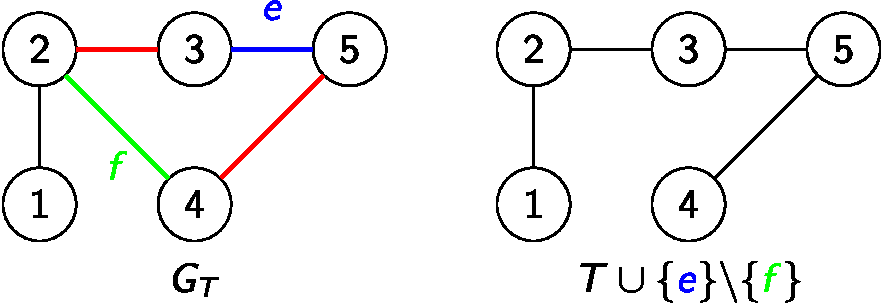
\includegraphics[width=.5\textwidth]{img/trees-5.pdf}
    \end{figure}

    \item Let $F$ be a partial tree (spanning nodes in $S \subseteq N$) contained in an optimal tree of $G$. Consider $e = \left\{u,v\right\} in \delta\left(S\right)$ of minimum cost, then there exists a minimum cost spanning tree of $G$ containing $e$ (is better explained in the \ref{paragraph: Prim's algorithm} paragraph, page \pageref{paragraph: Prim's algorithm}).

    \begin{proof}
        By contradiction, assume $T^{*} \subseteq E$ is a minimum cost spanning tree with $F \subseteq T^{*}$ and $e \notin T^{*}$. Adding edge $e$ to $T^{*}$ creates the cycle $C$. Let $f \in \delta\left(S\right) \cap C$.
        \begin{itemize}
            \item If $c_{e} = c_{f}$, then $T^{*} \cup \left\{e\right\} \setminus \left\{f\right\}$ is (also) optimal since it has same cost of $T^{*}$.
            
            \item If $c_{e} < c_{f}$, then $c\left(T^{*} \cup \left\{e\right\} \setminus \left\{f\right\}\right) < c\left(T^{*}\right)$, hence $T^{*}$ is not optimal.
        \end{itemize}
        \begin{figure}[!htp]
            \centering
            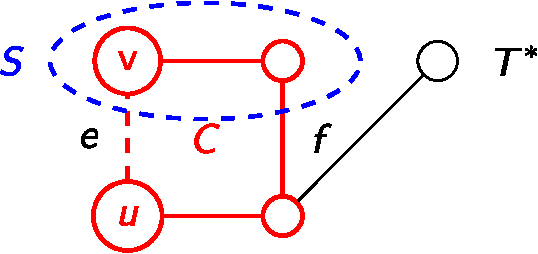
\includegraphics[width=.4\textwidth]{img/trees-9.pdf}
        \end{figure}
    \end{proof}
\end{enumerate}

\newpage

\subsubsection{Optimal cost spanning trees}

Spanning trees are very common because they are used in a wide range of applications such as network design, IP network protocols, enterprise storage, etc.

\begin{examplebox}[: introduction to finding the best and optimal cost solution]
    Design a communication network so as to connect $n$ cities at \textbf{minimum total cost}.

    The model is made up as follows:
    \begin{itemize}
        \item Graph $G = \left(N,E\right)$ with $n = \left| N \right|$, $m = \left| E \right|$
        \item Cost function $c: E \rightarrow c_{e} \in \mathbb{R}$, with $e = \left\{u,v\right\} \in E$.
    \end{itemize}
    \begin{center}
        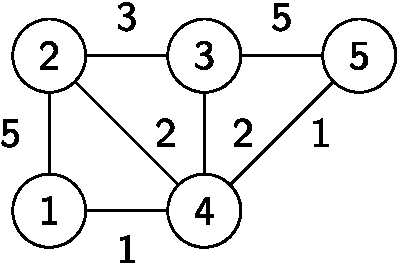
\includegraphics[width=.3\textwidth]{img/trees-6.pdf}
    \end{center}

    The required properties are:
    \begin{itemize}
        \item Each pair of cities must communicate, then the connected subgraph containing all the nodes.
        \item The minimum total cost, then the subgraph must have no cycles.
    \end{itemize}

    We give two solutions, where the second is better because it is more feasible and optimal:
    \begin{enumerate}
        \item $c\left(T_{1}\right) = 15$
        \begin{center}
            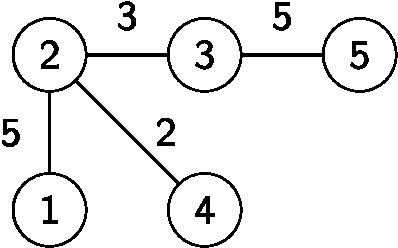
\includegraphics[width=.3\textwidth]{img/trees-7.pdf}
        \end{center}

        \item $c\left(T_{2}\right) = 6$
        \begin{center}
            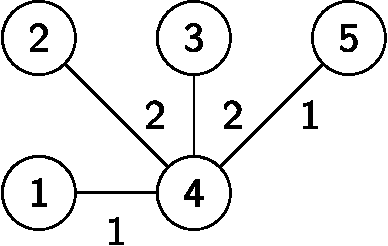
\includegraphics[width=.3\textwidth]{img/trees-8.pdf}
        \end{center}
    \end{enumerate}
\end{examplebox}

\newpage

\noindent
In general, we can formalize the \definitionWithSpecificIndex{optimal cost}{Optimal Cost} as follows. Given an undirected graph $G = \left(N,E\right)$ and a cost function, \textbf{find a spanning tree} $G_{T} = \left(N, T\right)$ \textbf{of minimum total cost}:
\begin{equation}
    \underset{T \in X}{\min} \displaystyle\sum_{e \in T} c_{e} \hspace{2em} \text{where } X \text{ is the set of all spanning trees of } G
\end{equation}

\highspace
Doesn't exists only one spanning tree, they are multiples. But the number of spanning trees available in a complete graph is defined by a theorem.
\begin{theorem}[Cayley, 1889]
    A complete graph with $n$ nodes ($n \ge 1$) has $n^{n-2}$ spanning trees.
\end{theorem}

\noindent
In general, the problem of finding a spanning tree with minimum total cost is also called \definitionWithSpecificIndex{minimum spanning tree (MST) problem}{minimum spanning tree (MST) problem}. It plays an important role in many networking applications, such as routing and networking.\cite{10.1007/978-3-642-38853-8_14}

\newpage

\paragraph{Prim's algorithm}\label{paragraph: Prim's algorithm}

\begin{definitionbox}[: Prim's]
    \definition{Prim's algorithm} is a \textbf{greedy algorithm that finds a minimum spanning tree for a weighted undirected graph}. This means it \textbf{finds a subset of the edges that forms a tree that includes every vertex, where the total weight of all the edges in the tree is minimized}. The algorithm operates by building this tree one vertex at a time, from an arbitrary starting vertex, at each step adding the cheapest possible connection from the tree to another vertex. Finally, \textbf{Prim's algorithm is exact} (it provides an optimal solution for every instance).
\end{definitionbox}

\highspace
A \definitionWithSpecificIndex{greedy algorithm}{Greedy algorithm} constructs a \textbf{feasible solution iteratively by making a \dquotes{locally optimal} choice at each step, without reconsidering previous choices}. In Prim's algorithm, at each step a minimum-cost edge is selected from those in the cut $\delta\left(S\right)$ induced by the current set of nodes $S$. Unfortunately, for most discrete optimization problems greedy-type algorithms yield a feasible solution with no guarantee of optimality.

\highspace
According to the definition of a greedy algorithm, the main idea of Prim is to build a spanning tree iteratively. It \textbf{starts with an initial tree} $\left(S,T\right)$ with $S = \left\{u\right\}$ ($u \in N$, so it can be any node in the set $N$) and $T = \emptyset$. At \textbf{each step}, \textbf{add} to the current sub-tree $\left(S,T\right)$ \textbf{a minimum cost edge} among those that connect a node in $S$ to a node in $N \setminus S$.

\begin{examplebox}[: Prim's algorithm]
    Suppose we have the following graph:
    \begin{center}
        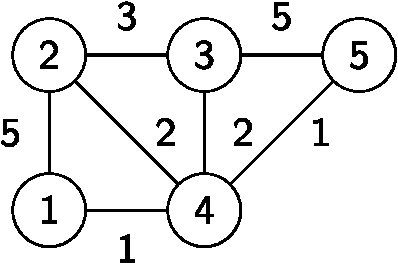
\includegraphics[width=.3\textwidth]{img/prims-alg-1.pdf}
    \end{center}

    \begin{enumerate}
        \item We start from an arbitrarily node $u$ that it is in the set $N$, for example $3$:
        \begin{center}
            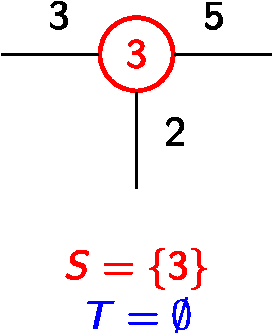
\includegraphics[width=.2\textwidth]{img/prims-alg-2.pdf}
        \end{center}

        \item As we said, at each step we add to the current subtree $\left(S, T\right)$ a minimum cost edge among those that connect a node in $S$ to a node in $N \setminus S$. So at this step we choose \emph{node 4} because the edge starting from \emph{node 3} is the less weighted edge.
        \begin{center}
            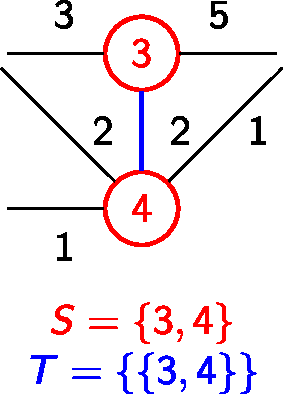
\includegraphics[width=.2\textwidth]{img/prims-alg-3.pdf}
        \end{center}

        \item At this point we continue with the same logic. The edge, starting from \emph{node 4}, with less weighted edge is \emph{node 1}. Note that at parity of the weighted edge, it doesn't matter which one we choose. Maybe the decision will lead to a different subgraph, but Prim's algorithm is greedy by definition, then it doesn't think about these problems; it assumes that it is a locally optimal choice.
        \begin{center}
            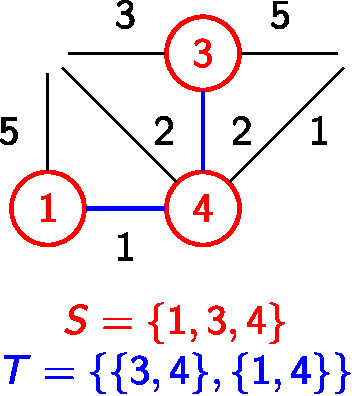
\includegraphics[width=.25\textwidth]{img/prims-alg-4.pdf}
        \end{center}

        \item Since we are lucky, the previous doubt is useless (with parity of weighted vertices, which should we choose?). Because \emph{node 1} exposes an edge with a weight of 5, but \emph{node 4} has a weighted edge of only 1, the choice is clear.
        \begin{center}
            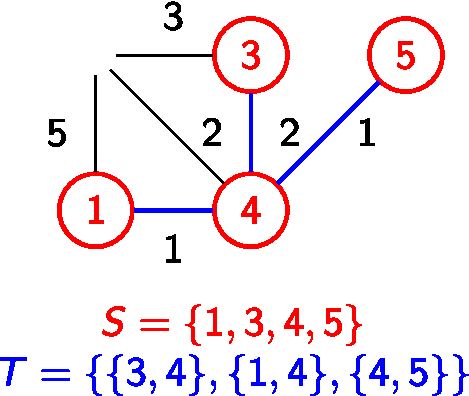
\includegraphics[width=.3\textwidth]{img/prims-alg-5.pdf}
        \end{center}

        \item Finally, we choose the edge with a weight of 2 (to the \emph{node 2}) because is the lowest. At this step, the algorithm is finished because there are no more vertices ($S = N$). The cost function returns the value $6$ (sum of each weighted edge selected).
        \begin{center}
            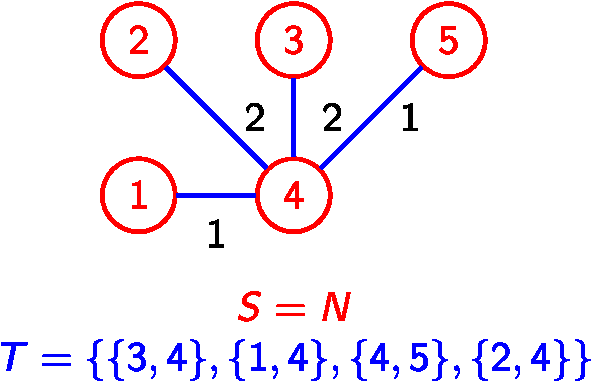
\includegraphics[width=.4\textwidth]{img/prims-alg-6.pdf}
        \end{center}
    \end{enumerate}
\end{examplebox}

\noindent
From the previous example it should be clear that at each step the Prim's algorithm creates the need to solve a minimum search problem.

\highspace
The Prim's algorithm take:
\begin{itemize}
    \item Input: a connected graph $G = \left(N,E\right)$ with edge costs.
    \item Output: a subset $T \subseteq N$ of edges of $G$ such that $G_{T} = \left(N,T\right)$ is a minimum cost spanning tree of $G$.
\end{itemize}

\begin{lstlisting}[language=pseudo-code, caption={Minimum spanning tree (MST) problem: Prim's $O\left(nm\right)$}]
S $\leftarrow$ $\{$u$\}$; $\label{prims: s-definition}$
T $\leftarrow$ $\emptyset$; $\label{prims: t-definition}$
while $\left|T\right| < n-1$ do: $\label{prims: while cycle}$
    $\left\{u\right\} \leftarrow$ edge in $\delta(S)$ of minimum cost; // with $u \in S$ and $v \in N \setminus S$ $\label{prims: search minimum}$
    $S \leftarrow S \cup \left\{v\right\}$; $\label{prims: add destination vertex}$
    $T \leftarrow T \cup \left\{\left\{u,v\right\}\right\}$ $\label{prims: add tuple source destination}$
\end{lstlisting}
\begin{itemize}
    \item[Rows \ref{prims: s-definition}-\ref{prims: t-definition}.] Declare the general sets $S$ and $T$. The first is filled with the starting node $u$ and the second is empty, because the core of the algorithm has not yet started.

    \item[Row \ref{prims: while cycle}.] Continue building the spanning tree until the length of the set of transitions $T$ is not equal to the number of nodes minus one.

    \item[Row \ref{prims: search minimum}.] Find the edge with the lowest weight from the set $\delta\left(S\right)$. Then choose one of the edges with the lowest weight and the corresponding target node. Obviously the target node $v$ cannot be already evaluated ($v \in N \setminus S$) and the source node $u$ must be in the set of nodes already evaluated ($u \in S$).
    
    \item[Rows \ref{prims: add destination vertex}-\ref{prims: add tuple source destination}.] Therefore, the most complex part of the algorithm (minimum search) is to store the target vertex with the lowest edge weight and add the tuple (source node, target node) to the set $T$.
\end{itemize}
The complexity of the algorithm is pretty much guessed. Or in the better case neither worst case, we need to evaluate each node. Then the main difference is made by the weighted edge search. If each edge has to be analyzed at each iteration, the \textbf{complexity} order is given by $O\left(nm\right)$.

\newpage

\paragraph{Implementation of Prim's algorithm in $O\left(n^{2}\right)$}

Prim's algorithm is based on graph traversals (visiting every vertex in the graph), which are inherently difficult to parallelize. It also has an irregular memory access pattern. In CPUs, this limits the use of the cache and leads to an overall performance penalty. The prim's algorithm is highly dependent on the organization of memory storage and memory access patterns.\cite{10.1007/978-3-642-38853-8_14}

\highspace
The following data structure we propose guarantees a complexity of $O\left(n^{2}\right)$.
\begin{itemize}
    \item $k$ is the number of edges selected so far;

    \item $S$ is the subset $S \subseteq N$ of nodes incident to the selected edges (same as explained in the \ref{paragraph: Prim's algorithm} section, page \pageref{paragraph: Prim's algorithm});
    
    \item $T$ is the subset $T \subseteq E$ of selected edges (same as explained in the \ref{paragraph: Prim's algorithm} section, page \pageref{paragraph: Prim's algorithm});
    
    \item $C_{j}$ is a vector which has a value equal to:
    \begin{equation*}
        C_{j} = \begin{cases}
            \min\left\{c_{ij} \: : \: i \in S\right\} & j \notin S \\
            \infty & \text{otherwise}
        \end{cases}
    \end{equation*}
    At the beginning of the algorithm it is clearly composed of infinite values if the edge $i$ to $j$ doesn't exist, otherwise the weight of the edge. In the core of the algorithm, each position is updated with the minimum weighted edge value.
    
    \item $\text{closest}_{j}$ is a vector which has a value equal to:
    \begin{equation*}
        \text{closest}_{j} = \begin{cases}
            \mathrm{argmin}\left\{c_{ij} \: : \: i \in S\right\} & j \notin S \\
            \text{predecessor of }j\text{ in the minimum spanning tree} & j \in S
        \end{cases}
    \end{equation*}
    The node closest to the edge has less weight, otherwise if we look at the node $j$ in the set $S$, the predecessor of that node in the minimum spanning tree. A trivial example:
    \begin{figure}[!htp]
        \centering
        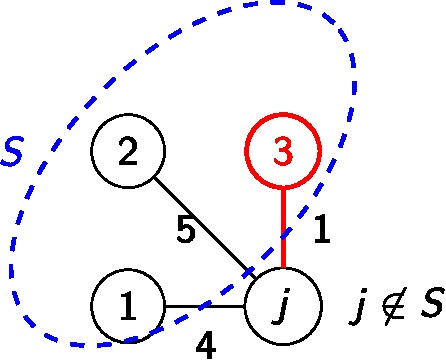
\includegraphics[width=.3\textwidth]{img/prims-alg-7.pdf}
    \end{figure}
    
    With $\mathrm{closest}_{j} = 3$ and $c_{\mathrm{closest}_{j}},j = 1$.
\end{itemize}
Let's take an example to clear up any doubts.

\begin{examplebox}[: Prim's algorithm $O\left(n^{2}\right)$]
    Suppose we have the following graph:
    \begin{center}
        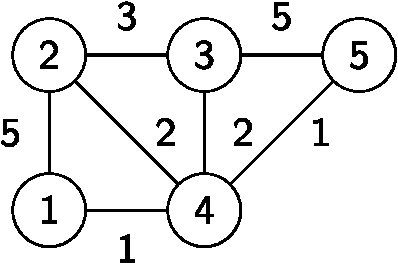
\includegraphics[width=.3\textwidth]{img/prims-alg-1.pdf}
    \end{center}

    \begin{enumerate}
        \item At the beginning we choose an arbitrary node $u$ that is in the set $N$, for example $3$. We set the set of transitions $T$ to the empty set, the set of evaluated nodes $S$ to the selected node $u$, in our case the value 3, and finally the two vectors. The vector $C_{j}$ is filled of infinite values if the edge $u$ to $j$ doesn't exist, otherwise the weight of the edge, and the vector $\text{closest}_{j}$ is filled with the selected starting node, in our case 3.
        \begin{itemize}
            \item $T = \emptyset$
            \item $S = \left\{u\right\} = \left\{3\right\}$
            \item $C_{j} = \left[+\infty, 3, -, 2, 5\right]$
            \item $\text{closest}_{j} = \left[3, 3, -, 3, 3\right]$
        \end{itemize}
        Some observations:
        \begin{itemize}
            \item The symbol $-$ is the \href{https://en.wikipedia.org/wiki/Don%27t-care_term}{don't care term used in digital logic}.
            \item The position of each value respects the j-index. For example, the node 3 in the vectors $C_{j}$ and $\text{closest}_{j}$ is placed at position number 3. The value is don't care ($-$) because it is the starting point. The other values depend on the graph. Node 1 has no direct edge to node 3, so it has an infty value; node 2 has a direct edge with weight 3; node 3 doesn't care because it's the starting point; and so on.
        \end{itemize}
        \begin{center}
            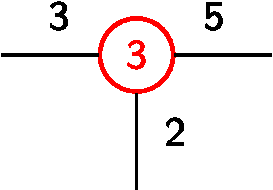
\includegraphics[width=.2\textwidth]{img/prims-alg-2-imp.pdf}
        \end{center}

        \item The minimum value in $C_{j}$ is 2 and since it is in the 4th position, node 4 is selected.
        \begin{itemize}
            \item $T = \left\{\left\{3,4\right\}\right\}$
            \item $S = \left\{3, 4\right\}$
            \item $C_{j} = \left[\mathbf{1}, \mathbf{2}, -, 2, \mathbf{1}\right]$
            \item $\text{closest}_{j} = \left[\mathbf{4}, \mathbf{4}, -, 3, \mathbf{4}\right]$
        \end{itemize}
        The values updated are the first, second and fifth positions, as nodes three and four are in the $S$ set.
        \begin{center}
            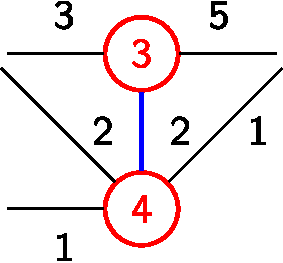
\includegraphics[width=.2\textwidth]{img/prims-alg-3-imp.pdf}
        \end{center}

        \item The minimum value in $C_{j}$ is the first position. But the fifth position is also the minimum. We choose the first value because the vector is analyzed sequentially (first to last).
        \begin{itemize}
            \item $T = \left\{\left\{3,4\right\}, \left\{1,4\right\}\right\}$
            \item $S = \left\{1, 3, 4\right\}$
            \item $C_{j} = \left[1, \mathbf{2}, -, 2, \mathbf{1}\right]$
            \item $\text{closest}_{j} = \left[4, \mathbf{4}, -, 3, \mathbf{4}\right]$
        \end{itemize}
        \begin{center}
            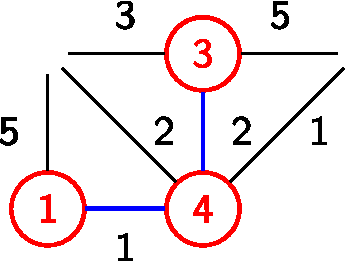
\includegraphics[width=.25\textwidth]{img/prims-alg-4-imp.pdf}
        \end{center}

        \item The minimum value in $C_{j}$ is quite trivial, between 2 and 1. We choose the value 1 and the node $4$ is the closest.
        \begin{itemize}
            \item $T = \left\{\left\{3,4\right\}, \left\{1,4\right\}, \left\{4,5\right\}\right\}$
            \item $S = \left\{1, 3, 4, 5\right\}$
            \item $C_{j} = \left[1, \mathbf{2}, -, 2, 1\right]$
            \item $\text{closest}_{j} = \left[4, \mathbf{4}, -, 3, 4\right]$
        \end{itemize}
        \begin{center}
            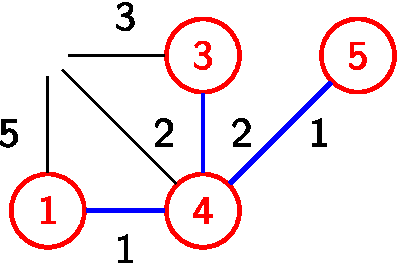
\includegraphics[width=.3\textwidth]{img/prims-alg-5-imp.pdf}
        \end{center}

        \item Finally, node 2 with edge weight 2 is selected.
        \begin{itemize}
            \item $T = \left\{\left\{3,4\right\}, \left\{1,4\right\}, \left\{4,5\right\}, \left\{2,4\right\}\right\}$
            \item $S = \left\{1, 2, 3, 4, 5\right\} = N$
            \item $C_{j} = \left[1, 2, -, 2, 1\right]$
            \item $\text{closest}_{j} = \left[4, 4, -, 3, 4\right]$
        \end{itemize}
        \begin{center}
            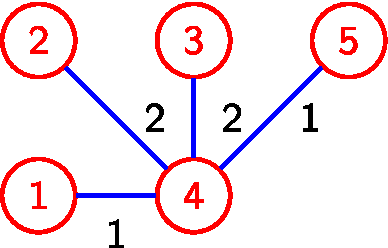
\includegraphics[width=.3\textwidth]{img/prims-alg-6-imp.pdf}
        \end{center}
    \end{enumerate}
\end{examplebox}

\noindent
\begin{flushleft}
    \textcolor{Green3}{\faIcon{question-circle} \textbf{Ok, but how do we get the spanning tree from the nearest vector?}}
\end{flushleft}
The minimum spanning tree found by Prim's algorithm consists of the $n-1$ edges:
\begin{equation*}
    \left\{\text{closest}_{j}, j\right\} \hspace{2em} \text{with } j = 1,2,\dots,n
\end{equation*}
For example, from the previous example, let the \emph{closest} vector:
\begin{equation*}
    \text{closest}_{j} = \left[4,4,-,3,4\right]
\end{equation*}
A minimum cost spanning tree consists of the edges:
\begin{equation*}
    \left\{4,1\right\}, \left\{4,2\right\}, \cancel{\left\{-,-\right\}}, \left\{3,4\right\}, \left\{4,4\right\}
\end{equation*}
\begin{lstlisting}[language=pseudo-code, caption={Minimum spanning tree (MST) problem: Prim's $O\left(n^{2}\right)$}]
S $\leftarrow$ $\{$u$\}$; $\label{prims-imp: s-definition}$
T $\leftarrow$ $\emptyset$; $\label{prims-imp: t-definition}$
for $j \in N \setminus S$ do: $\label{prims-imp: for j in N setminus S}$
    $C_{j} \leftarrow c_{uj}$; // or $+\infty$ if $\left\{u,j\right\} \notin E$
    $\text{closest}_{j} \leftarrow u$; $\label{prims-imp: end for}$
for $k = 1, \dots, n-1$ do: $\label{prims-imp: for k from 1 to n-1}$
    // select min edge in $\delta(S)$
    min $\leftarrow +\infty$; $\label{prims-imp: start select minimum edge}$
    for $j = 1, \dots, n$ do: $\label{prims-imp: third for}$
        if $j \notin S$ and $C_{j} <$ min:
            min $\leftarrow C_{j}$;
            v $\leftarrow$ j; $\label{prims-imp: end select minimum edge}$
    // extend S and T
    S $\leftarrow$ S $\cup \left\{v\right\}$; $\label{prims-imp: start extend S and T}$
    T $\leftarrow$ T $\cup \left\{\left\{\text{closest}_{v}, v\right\}\right\}$; $\label{prims-imp: end extend S and T}$
    // update $C_{j}$ and $\text{closest}_{j}$, $\forall j \notin S$
    for $j = 1, \dots, n$ do: $\label{prims-imp: for j from 1 to n}$
        if $j \notin S$ and $c_{vj} < C_{j}$:
            $C_{j} \leftarrow c_{vj}$;
            $\text{closest}_{j} \leftarrow v$; $\label{prims-imp: end for j from 1 to n}$
\end{lstlisting}
\begin{itemize}
    \item[Rows \ref{prims-imp: s-definition}-\ref{prims-imp: t-definition}.] Declare the general sets $S$ and $T$. The first is filled with the starting node $u$ and the second is empty, because the core of the algorithm has not yet started.

    \item[Rows \ref{prims-imp: for j in N setminus S}-\ref{prims-imp: end for}.] The first for statement is used to initialize the two vectors $C_{j}$ and $\text{closest}_{j}$. It inserts the edge weight into $C_{j}$ if there is a direct edge from $u$ to $j$, otherwise infinity is used. Meanwhile, the \emph{closest} vector consists only of the starting node $u$ at the beginning of the algorithm.

    \item[Row \ref{prims-imp: for k from 1 to n-1}.] The second for statement is the core of the algorithm. Here the index goes from one to the number of nodes minus one.
    
    \item[Rows \ref{prims-imp: start select minimum edge}-\ref{prims-imp: end select minimum edge}.] This piece of code is used to select the minimum edge available in the $C_{j}$ vector. It starts by setting the \texttt{min} variable to infinity, to ensure that a value is selected. Therefore, the for statement iterates over each node; at each iteration, if the selected node is not in the $S$ set (so it has not already been evaluated) and the value at the corresponding position in the vector $C_{j}$ is less than minimum, then assign to the minimum the value of the vector $C_{j}$ at position $j$ and to $v$ the index $j$.

    \item[Rows \ref{prims-imp: start extend S and T}-\ref{prims-imp: end extend S and T}.] Now it updates the variable $S$ with the node $v$ and the transitions set with the tuple (value at the corresponding position in the vector $\text{closest}_{v}$, node $v$).

    \item[Rows \ref{prims-imp: for j from 1 to n}-\ref{prims-imp: end for j from 1 to n}.] There is another for statement similar to the previous one, because here it needs to update the vectors $C_{j}$ and $\text{closest}_{j}$ with the new values. The for iterates over every node of the graph. So at each iteration it checks that the selected vertex is not in the $S$-set (not already evaluated) and that the weight of the edge from vertex $v$ to $j$ (if it exists, otherwise infinity) is less than the value $C_{j}$. If the double condition is true, it updates the two vectors at position $j$.
\end{itemize}
The overall complexity is given by:
\begin{itemize}
    \item The number of iterations of the first for at row \ref{prims-imp: for j in N setminus S}, which is: $\left(n-1\right)$

    \item Plus the number of iterations of the second for at row \ref{prims-imp: for k from 1 to n-1}, which is: $\left(n-1\right)$
    
    \item Times the number of iterations of the third and fourth for at lines \ref{prims-imp: third for} and \ref{prims-imp: for j from 1 to n}, which is: $\left(n-1+n-1\right)$
\end{itemize}
The result is $O\left(n^{2}\right)$. For sparse graphs, a more sophisticated data structure leads to an $O\left(m \log n\right)$ complexity.

\longline

\paragraph{Optimality condition}

Given a spanning tree $T$, an \textbf{edge} $e \notin T$ is \definitionWithSpecificIndex{cost decreasing}{Edge cost decreasing} if when $e$ is added to $T$ it creates a cycle $C$ with $C \subseteq T \cup \left\{e\right\}$ and $\exists f \in C \setminus \left\{e\right\}$ such that $c_{e} < c_{f}$.
\begin{figure}[!htp]
    \centering
    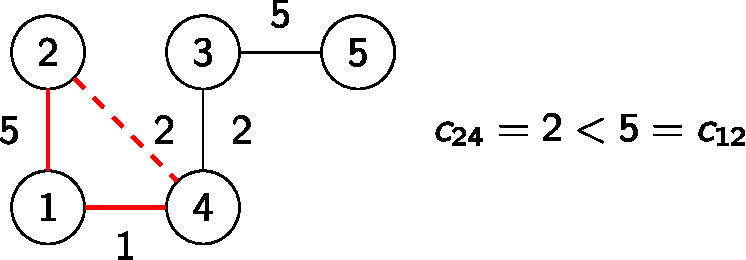
\includegraphics[width=.5\textwidth]{img/trees-opt-condition.pdf}
\end{figure}

\noindent
Because $c\left(T \cup \left\{e\right\} \setminus \left\{f\right\}\right) = c\left(T\right) + c_{e} - c_{f}$, if $e$ is cost decreasing, then:
\begin{equation*}
    c\left(T \cup \left\{e\right\} \setminus \left\{f\right\}\right) < c\left(T\right)
\end{equation*}
\begin{theorem}[Tree optimality condition]
    A tree $T$ is of minimum total cost if and only if no cost-decreasing edge exists.
\end{theorem}
\begin{proof}
    $\Rightarrow$ If a cost-decreasing edge exists, then $T$ is not of minimum total cost.

    $\Leftarrow$ if no cost-decreasing edge exists, then $T$ is of minimum total cost. Let $T^{*}$ be a minimum cost spanning tree found by Prim's algorithm. It can be verified that, by exchanging one edge at a time, $T^{*}$ can be iteratively transformed into $T$ without modifying the total cost. Thus, $T$ is also optimal.
\end{proof}

\noindent
Testing optimality is quite simple. The optimality condition allows to verify whether a spanning tree $T$ is optimal: it suffices to check that each $e \in E \setminus T$ is not a cost-decreasing edge.

    %%%%%%%%%%%%%%%%%%%
    % Fancy pagestyle %
    %%%%%%%%%%%%%%%%%%%
    \pagestyle{fancy}
    \fancyhead{} % clear all header fields
    \fancyhead[R]{\nouppercase{\leftmark\hfill\rightmark}}

    %%%%%%%%%%%%%%%%%%%%%%%%%%
    % Bibliography and index %
    %%%%%%%%%%%%%%%%%%%%%%%%%%
    \pagestyle{fancy}
\fancyhead{} % clear all header fields
\fancyhead[R]{\nouppercase{\leftmark}}

\bibliography{bibtex}{}
\bibliographystyle{plain}

\newpage

\printindex
\end{document}